\subsection{Performance Requirements}
\begin{itemize}
	
\end{itemize}
\subsection{Design Constraints}
\begin{enumerate}
	
\end{enumerate}
\subsection{Software System Attributes}



\subsection{Class diagram}
 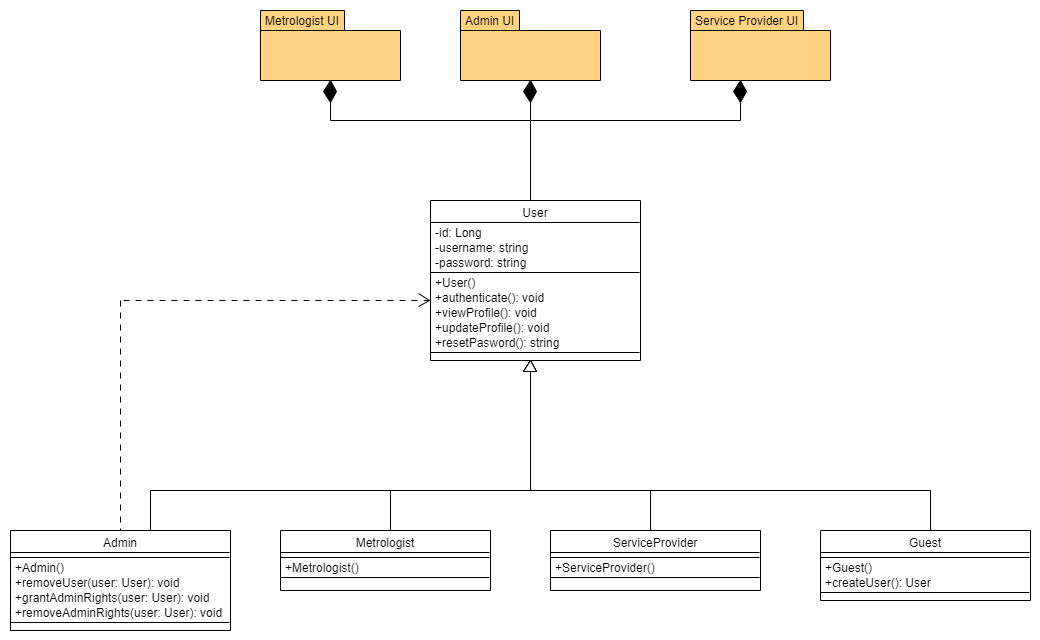
\includegraphics[width=12cm,height=26cm,keepaspectratio]{users_unit/Images/users class diagram.png}
	\begin{center}
	    \small{Figure #: Class diagram for ...}
    \end{center}
\paragraph{Design Patterns Used}
	
	
		
\subsection{Activity diagram}
    %\includegraphics[width=\textwidth]{}
	\begin{center}
	    \small{Figure #: Activity diagram for ...}
    \end{center}


\subsection{Sequence diagram}
    %\includegraphics[width=\textwidth]{}
	\begin{center}
	    \small{Figure #: Sequence diagram for ...}
    \end{center}

\subsection{State diagram}
    %\includegraphics[width=\textwidth]{}
	\begin{center}
	    \small{Figure #: State diagram for ...}
    \end{center}




\subsection{Use Case diagram}
    %\includegraphics[width=\textwidth]{}
    \begin{center}
    	\small{Figure #: Use case diagram for ...}
    \end{center}